\chapter{Geometri}
I lineær programmering afsnittet, er løsningerne til et optimeringsproblem beskrevet som værende alle de $\vec{x}$ som overholder bibetingelserne. Dette er beskrevet som værende et polyhedron.
\begin{defn} [Polyhedron]
Et \textbf{Polyhedron} er en mængde 
\begin{align*}
 P =\{ \vec{x} \in \mathds{R}^n | A \vec{x} \geq \vec{b}, \vec{b}\in \mathds{R}^m\},
\end{align*}
hvor at $A$ er en $m \times n$ matrice.
\end{defn}
Hvis et lineært programmerings problem står på standard form $\{ \vec{x} \in \mathds{R}^n | A \vec{x} = \vec{b}, \vec{b}\in \mathds{R}^m\}$, så kaldes dette stadig et polyhedron.\\

Hvis der er en polyhedron $P=\{x|A\vec{x}=\vec{b},x\geq 0\}$ som består af alle bibetingelserne for problemet, så må der også findes en anden polyhedron $Q$, som består af alle de lineære uafhængige bibetingelserne for problemet. Det giver god mening, at fordi $P$ består af de samme bibetingelser som $Q$ og så lidt flere til, så er en løsning $\vec{x}$ til $P$ også en løsning til $Q$ og modsat er en løsning til $Q$ også en løsning til $P$ og derfor må $Q=P$, hvilket vil blive bevist i følgende sætning.

\begin{stn} 
Lad $P=\{\vec{x}|A\vec{x}=\vec{b},x\geq 0\}$ være en ikke-tom polyhedron, hvor $A$ er en $m\times n$ matrix med lineære uafhængige søjler.\\
Antag at $rank(A)=k<m$. Betragt polyhedronen $Q=\{\vec{x}|A_{j_1}\vec{x}=b_{i_1},\dots ,A_{j_k}\vec{x}=b_{i_k}\}$, så er $Q=P$.
\label{stn:PQ}
\end{stn}
\begin{proof}
Hvis $P=\{x|A\vec{x}=\vec{b},x\geq 0\}$ er en polyhedron, der består af alle bibetingelserne og har $rank(A)=k$, så må der være en $Q=\{\vec{x}|A_{j_1}\vec{x}=b_{i_1},\dots ,A_{j_k}\vec{x}=b_{i_k}\}$, der består af alle lineære uafhængig bibetingelser. Så må $P\subset Q$, eftersom alle elementerne i $P$ også tilfredsstiller bibetingelserne for $Q$.\\
Eftersom $rank(A)=k$, så er $k$ rækkerummet af $A$ og så former rækkerne $\vec{a_1},\dots ,\vec{a_k}$ en basis for rækkerummet, derfor kan lineare kombinationen af rækkerne $a_i$ af $A$, skrives som $a_i=\sum_{j=1}^{k}{i j}\vec{a_j}$ for en skalar $c_{i j}$, lad så $\vec{x}$ være en del af $P$ så
\begin{align*}
\vec{a_i}\vec{x}=\sum_{j=1}^{k}c_{i j}\vec{a_j}\vec{x}=\sum_{j=1}^{k}c_{i j}\vec{b_j}=\vec{b_i} \qquad i=1,\dots,m.
\end{align*}
Lad nu $\vec{y}$ være en del af Q, så er $\vec{y}$ også en del af P, eftersom:
\begin{align*}
\vec{a_i}\vec{y}=\sum_{j=1}^{k}c_{i j}\vec{a_j}\vec{y}=\sum_{j=1}^{k}c_{i j}\vec{b_j}=\vec{b_i} \qquad i=1,\dots,m.
\end{align*}
Hvilket betyder $\vec{y}\in P$ og $Q\subset P$ og derved $P=Q$.
\end{proof}

\section{Basisløsninger}

%Jeg har endnu ikke fået gennemgået beviserne til de to sætninger ordentligt. de er bare stjålet fra jer andre.

Basisløsninger danner grundlaget for udregningen af den optimale løsning, hvilket beskrives og anvendes i Kapitel \ref{afsnit:simplex}. For at kunne beskrive netop basisløsninger er det nødvendigt først at introducere definitionen for \textbf{aktive betingelser}.%Ved ikke: Skal vi også bruge fed når ord introduceres i bindende tekst?

\begin{defn}[Aktive betingelser]
En betingelse siges at være \textbf{aktiv} for en givet løsningsvektor $\vec{x}$, hvis det gælder, at\\ $\vec{a}_i^T \vec{x}^* = b_i$.
\label{def:aktiv}
\end{defn}

Generelt bliver aktive betingelser brugt, da de for uligheder repræsenterer en grænse for de mulige løsninger i en given retning, mens de for ligheder blot beskriver, at betingelsen er opfyldt.
Yderligere anvendes skæringen mellem disse aktive betingelser, da den optimale løsning for lineære programmeringsproblemer findes i netop disse skæringer. Hvorfor dette netop er tilfældet bliver begrundet i Afsnit \ref{sec:eksistens}.

\begin{stn}[Lineært uafhængige rækker]
Lad $\vec{x}^* \in \mathds{R}^n$ og $I = \{i | \vec{a_i}^T \vec{x}^* = b_i\}$ være mængden af indekser for aktive betingelser. Da er følgende ækvivalent
\begin{enumerate}[label=(\alph*)]
\item Mængden $R_a =\{\vec{a_i}| i\in I\}$ indeholder vektorer, hvoraf $n$ af dem er lineært uafhængige.
\item Spannet $span(R_a) = \mathds{R}^n$.
\item Ligningssystemet $\vec{a_i}^T \vec{x}^* = b_i$, for $i \in I$ har en unik løsning.
\end{enumerate}
\label{stn:uniklosning}
\end{stn} %Ved ikke: Bør det siges at $\vec{a_i}$ repræcentere en række, eller er det underforstået i rapporten da den altid gør det?

\begin{proof}
	(a) <=> (b): Antag at der i $R_a$ er $n$ lineært uafhængige vektorer. Da der er $n$ lineært uafhængige vektorer må dimensionen af spannet af $R_a$ være $n$. Da $dim(span(R_a))=dim(\mathds{R}^n)=n$ og da $R_a \subseteq \mathds{R}^n$ må det følge af Sætning \ref{stn:dimunderrum} at $span(R_a)=\mathds{R}^n$. Tilsvarende gælder det at hvis $span(R_a)=\mathds{R}^n$, må det gælde at $dim(span(R_a))=dim(\mathds{R}^n)=n$. Da vil kardinaliteten af en basis for $R_a$ nødvendigvis være $n$, hvorved $R_a$ skal indeholde $n$ lineært uafhængige vektorer.


(a) <=> (c): Antag at $span(R_a)=\mathds{R}^n$. Antag nu for modstrid at der findes to løsninger, $\vec{x}_a$ og $\vec{x}_b$ som opfylder $\vec{a}_i\vec{x}=\vec{b}$ for alle $i \in I$. 
Da vil det for alle $i \in I$ gælde at $\vec{a}_i^T\vec{x}_a=\vec{b}$ og at $\vec{a}_i^T\vec{x}_b=\vec{b}$, hvorved $\vec{a}_i^T\vec{d}=\vec{0}$, hvor $\vec{d}=\vec{x}_a-\vec{x}_b$. 
Vektoren $\vec{d}$ vil da være orthogonal på alle $\vec{a}_i$ for $i \in I$ og kan derfor ikke være en lineær kombination af disse. Herved kan $R_a$ ikke udspænde hele $\mathds{R}^n$, da $\vec{d} \in \mathds{R}^n$ men $\vec{d} \notin span(R_a)$.
Tilsvarende antages det nu at der kun er en unik løsning til ligningssystemet. For modstrid antages det at $R_a$ ikke udspænder hele $\mathds{R}^n$ Der kan derved vælges en vektor $\vec{d}$ som er orthogonal til $span(R_a)$ hvorved $\vec{a}_i^T(\vec{x}+\vec{d})=\vec{b}$. derved er $\vec{x}$ ikke en unik løsning og der er opstået modstrid.
\end{proof}
	
	
	
	%Da er disse vektorer en basis for det underrum af $\mathds{R}^n$, som de udspænder. Da $dim(\mathds{R}^n)=dim(R_a)=n$ medfører det af sætning [4.59] at $span(R_a)=\mathds{R}^n$. Tilsvarende gælder det at hvis $span(R_a)=\mathds{R}^n$, må det gælde at $dim(span(R_a))=dim(\mathds{R}^n)=n$. Da vil kardinaliteten af en basis for $R_a$ nødvendigvis være $n$, hvorved $R_a$ skal indeholde $n$ lineært uafhængige vektorer.



%\begin{proof}
%(a) => (c): Lad $A$ være en $n \times n$ matrix bestående af rækkerne $\vec{a_i} \in R_a$, og antag at alle $\vec{a_i}$ er lineært uafhængige. 
%Antag nu for modstrid at ligningssystemet $A\vec{x} = \vec{b}$, hvor $\vec{b}$ har indgangende $b_i$ for $i \in I$, har to løsninger. 
%Da vil $A \vec{x} = \vec{b}$ og $A \vec{y} = \vec{b}$ hvorfor $A(\vec{x}-\vec{y}) = \vec{0}$.
%Derfor må søjlerne enten være lineært afhængige, eller $(\vec{x}-\vec{y})= \vec{0}$.
%Da der er $n$ lineært uafhængige rækker i $A$ må $rank(A) = n$, hvorfor alle søjler er lineært uafhængige, da $A$ er en $n \times n$ matrix.
%Det medfører at $\vec{x}-\vec{y} = \vec{0}$, hvorfor det kan konkluderes at løsningen til ligningssystemet er unikt da $ \vec{x}=\vec{y}$, og der derved er bevist modstrid.
%\\(c) => (a): Antag at der er en unik løsning til $A\vec{x} =\vec{b}$. Det medfører at der er en pivotindgang i hver række hvorved: $rank(A) = n$. hvorfor alle rækker må være lineært uafhængige, da $A$ er en $n \times n$ matrice. % s. 78-79 LinAlg
%\\ (a) => (b): Da $R_a$ består af $n$ linært uafhængige $n$-dimentionelle vektorer, må $R_a$ udgøre en base for $\mathds{R}^n$, hvorfor $span(R_a) = \mathds{R}^n$.
%\\ (b) => (a): Antag for modstrid, at vektorene i $R_a$ ikke er lineært uafhængige, da vil der eksistere en vektor $\vec{a}_i \in R_a$ som er en linear kombination af de andre vektorer, der må derfor eksistere en vektor $A\vec{x} = \vec{0}$, hvor $\vec{x} \neq \vec{0}$.
%Da det kun kan lade sig gøre hvis $\vec{x}$ er ortogonal med alle rækker i $A$, kan $\vec{x}$ ikke være en linear kombination af vektorene i $R_a$.
%Hvorfor at $\vec{x} \notin span(R_a)$.
%Derfor kan $span(R_a) \neq \mathds{R}^n$, hvorfor der er opstået modstrid.
%\end{proof}

\begin{defn}[Basisløsning]
Lad $P$ være en polyide dannet af lineære bibetingelser, og lad $\vec{x}^*\in \mathds{R}^n$. Da er $\vec{x}^*$ en \textbf{basisløsning} hvis
\begin{enumerate}[label=(\alph*)]
\item Alle lighedskrav er aktive
\item Der er $n$ lineært uafhængige aktive betingelser
\end{enumerate}
og en \textbf{mulig basisløsning} hvis
\begin{enumerate}[label=(\alph*)]
\setcounter{enumi}{2}
\item $\vec{x}^*$ opfylder alle krav.
\end{enumerate}
\label{def:basislosning}
\end{defn}

Enhver bibetingelse udspænder et rum, for hvilket betingelsen er opfyldt. Skæringen, af de aktive betingelser, danner derved et rum, som er fællesmængden, af betingelsernes udspændte rum. Skæringen, af en mængde af aktive betingelser, svarer derved til den mulige mængde af disse betingelser. Dog gælder det for basisløsninger pr. Definition \ref{def:basislosning}, at der for en basisløsning $\vec{x}$ skal være $n$ lineært uafhængige aktive betingelser, hvorved en basisløsningen er en unik vektor, hvilket er bevist igennem Sætning \ref{stn:uniklosning}. %Ved ikke, er en vektor og et punkt det samme?

\begin{kor}[Endelig mængde af basisløsninger]
Givet en endelig mængde af bibetingelser, vil der kun eksistere en endelig mængde af basisløsninger og derved også kun en endelig mængde mulige basisløsninger.
\end{kor}

\begin{proof}
Betragt et lineært ligningssystem med $m$ uligheder og løsningsvektorer på formen $\vec{x} \in \mathds{R}^n$, hvor m er et endelige tal.
	Betragt da systemet af $n$ aktive uafhængige lineære uligheder udvalgt af de $m$ uligheder. Da vil dette system ifølge Sætning \ref{stn:uniklosning} kun have en løsning, og denne udvælgelse af uligheder giver derved kun en basisløsning. Da der kun er en endelig mængde af muligheder for at udtrække $n$ af $m$ uligheder på, vil der netop også kun være en endelig mængde af basisløsninger. Da mængden af mulige basisløsninger er en delmængde af mængden af basisløsninger, vil der også kun være en endelig mængde af mulige basisløsninger.
\end{proof}

\begin{stn}[Krav til basisløsninger]
Lad $A\vec{x}=b$, $\vec{x}\geq 0$, hvor $A$ er en $m\times n$ matrix med lineært uafhængige rækker. Da er $\vec{x}^*\in \mathds{R}^n$ en basisløsning hvis og kun hvis $A\vec{x}^*=b, \vec{x}^* \geq 0$, og der eksisterer indekser $B(1), ..., B(m)$ således, at
\begin{enumerate}[label=(\alph*)]
\item Kolonerne $A_{B(1)}, ..., A_{B(m)}$ er lineært uafhængige
\item $x_j = 0$ hvis $j \neq B(1),...,B(m)$.
\end{enumerate}
\end{stn}

\begin{proof}
Først vises at (a) og (b) medfører at $\vec{x}$ er en basisløsning.
Lad $I_m$ være mængden af indeks for de lineært uafhængige søjler  $I_m=\{B(1),\dots,B(m)\}$. Per definition er $\vec{b}=\sum_{j=1}^{n} x_j \vec{A}_j$, hvilket må være det samme som $\vec{b}=\sum_{j\in I_m} x_j \vec{A}_j+\sum_{j\notin I_m} x_j \vec{A}_j$, hvor summeringen er opdelt efter om kolonnerne har indeks $i \in I_m$. 
Ifølge sætningens punkt (b) er $x_j=0$ for $j \notin I_m$. Derved bliver summeringen forkortet til $\vec{b}=\sum_{j\in I}x_j \vec{A}_j$. Da vektorerne $\vec{A}_j$ for $j \in I_m$ er lineært uafhængige vil ligningssystemet nødvendigvis have en unik løsning. Da der er $m$ aktive betingelser, vil det pr. Definition \ref{def:basislosning} at $\vec{x}$ er en basisløsning.

% som er summen af alle de lineære uafhængige rækker og deres løsninger lagt sammen med summen af de lineære afhængige rækker og deres løsninger, men $\vec{x_j}$ til de lineære uafhængige løsninger er er i følge sætningen $x_i = 0$ hvis $i \neq B(1),...,B(m)$ så derfor må ligningen blive $b=\sum_{j\in I_m}^{n}x_j \vec{A}_j+0$,
% 
%så derfor må $\vec{x}$ være en basis løsning.

Herefter vises at det at $\vec{x}$ er en basisløsning medfører (a) og (b). Antag at $\vec{x}$ er en basisløsning og lad $x_j$ for indekser $j \in I_k=\{B(1),\dots B(k)\}$ være alle ikke-nul komponenter af $\vec{x}$.
Eftersom $\vec{x}$ er en basisløsning, så må ligningssystemet af aktive betingelser $\sum_{j=1}^{n}\vec{A}_jx_j=\vec{b}$, hvor $x_j=0$ for $j\notin I_k$ have en unik løsning. Dette gælder da en basisløsning har $n$ uafhængige aktive betingelser, hvilket ifølge Sætning \ref{stn:uniklosning} medfører at systemet har en unik løsning. 
Ligeledes må ligningen $\sum_{j \in I_k}\vec{A}_jx_j=\vec{b}$ have en unik løsning og derfor må kolonerne $\vec{A}_{B(1)}, ..., \vec{A}_{B(k)}$ være lineært uafhængige. Derfor må det gælde at $k \leq m$. % Hvis ikke dette var tilfældet ville der eksistere flere $\vec{x}$ som opfylder ligningssystemet, hvilket modstrider at der er en unik løsning.\\
%Eftersom kolonerne $\vec{A}_{B(1)}, ..., \vec{A}_{B(k)}$ er lineært uafhængige, så må det gælde at $k\leq m$. 
Da $A$ har $m$ lineært uafhængige rækker, må $A$ også have $m$ lineært uafhængige kolonner, hvorved $Col(A)=\mathds{R}^m$.

Den næste del af beviset viser, at der for enhver udvælgelse af indekser $I_k$ findes indekser $I_m$ således at $I_k \subseteq I_m$. 
%Den næste del af beviset viser, at der for enhver udvælgelse af $k$ lineært uafhængige kolonner med indekser $I_k$, gælder at der findes en mængde af $m$ lineært uafhængige kolonner med indekser $I_m$, hvorom det gælder at $I_k \subseteq I_m$.
Altså findes der indekser $B(k+1),...,B(m)$, således at kolonnerne med indekser $B(1),...,B(k),...,B(m)$ er lineært uafhængige. 

Hvis alle $\vec{A}_j$ for $j \notin I_k$ er lineært afhængige af $\vec{A}_j$ for $j \in I_k$, gælder det at $span\left( \vec{A}_{B(1)},...,\vec{A}_{B(k)} \right)=Col(A)=\mathds{R}^m$, hvorved $k=m$. 
Hvis der i stedet eksisterer en kolonne med indeks $j \notin I_k$ som er lineært uafhængig af disse kolonner, kan denne tilføjes til mængden af nu $k+1$ uafhængige vektorer. Denne proces kan gentages $m-k$ gange. Da $i \notin I_m$ medfører at $i \notin I_k$ gælder det derved at $\vec{x}_i =0$ for $i \notin I_m$
\end{proof}

\begin{pro}[Procedure for konstruktion af basisløsninger]
\noindent 1. Vælg $m$ lineært uafhængige koloner $\vec{A}_{B(1)},\dots,\vec{A}_{B(m)}$\\
2. Lad $x_i=0 \,\forall i\neq B(1),\dots,B(m)$\\
3. Løs $A\vec{x}=\vec{b}$ for de ubekendte $x_{B(1)},\dots x_{B(m)}$
\end{pro}

\begin{comment}
Der mangler bare generelt bindetekst mellem sætninger, fra at korollar 6.12 skal introduceres til at kapitlet skal afsluttes og føres videre til naboløsninger
\end{comment}

\subsection{Naboløsninger}

Til den senere anvendelse af simpLeX metoden anvendes også \textbf{naboløsninger}, som er defineret i Definition \ref{def:nabo}. Undersøgelsen af naboløsninger i simpLeX metoden som en metode til at reducere antallet af basisløsninger som skal undersøges når den optimale løsning findes. %Bør omformuleres, er kringlet. Ved ikke: Er det realt det der sker? Ved ikke: Skal SimpLeX staves med stort? Jeg tror da det er det der sker. og simplex er med lille. hermed rettet.

\begin{defn}[Naboløsninger]
	To basisløsninger i $\mathds{R}^n$ siges af være \textbf{naboløsninger}, hvis de deler præcis $n-1$ aktive lineært uafhængige bibetingelser.
	\label{def:nabo}
\end{defn}

Et eksempel på naboløsninger ses i Eksempel \ref{eks:nabo}.

\begin{eks}[Naboløsninger]
De to basisløsninger $\vec{p}=\rvect{4 & 4}^T$ og $\vec{q}=\rvect{10 & 2}^T$ set på Figur \ref{fig:nabo} er naboløsninger, da de har $n-1$ fælles aktive betingelser, hvilket for dette eksempel er 1 betingelse, nemlig betingelse (2). Basisløsningen $\vec{p}$ har (1) og (2) som aktive betingelser, mens $\vec{q}$ har (2) og (3) som aktive betingelser. %ved ikke, om nemlig bør slettes.
	
	\begin{center}
	\begin{tabular}{l	>{$}r<{$}	>{$}r<{$}	>{$}l<{$} r}
	Maksimer 		& 		4x_1	&	+3 x_2	& \\
	med hensyn til 	&  \ \ 	-2 x_1	& 	+4 x_2	& \leq 8 	& \quad (1)\\
					&  		x_1		& 	+3 x_2	& \leq 16	& \quad (2)\\
					&  \ \ 	x_1		& 			& \leq 10	& \quad (3)\\
	og $x_1 \geq 0$ (4), $x_2\geq 0$ (5).
	\end{tabular}
	\end{center}
	
	\begin{center}
	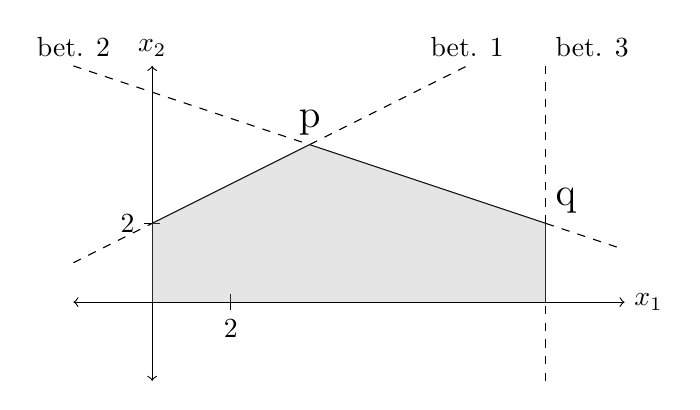
\begin{tikzpicture}
  %laver Grid. godt til når koordinater skal redigeres
  	%\draw[thin,gray!40] (-3,-1) grid (6,3); 
  %x-aksen
  	\draw[<->] (-1,0)--(6,0) node[right]{$x_1$};
  	%\draw[->,red] (2.5,0) -- (2.5,0.5);
  %y-aksen
  	\draw[<->] (0,-1)--(0,3) node[above]{$x_2$};
  	%\draw[->,red] (0,0.5) -- (0.5,0.5);
  	
  %akse-markeringer
  	%\node[left] (xakse) at (0,1) {2};
  	\draw[] (-0.1,1) -- (0.1,1) node[pos=0,left] {2};
  	\draw[] (1,-0.1) -- (1,0.1) node[pos=0,below] {2};
  	
  %ligning 1
	\draw[domain=-1:0,variable=\x,dashed] 	plot({\x},{0.5*\x+1});
	\draw[domain=0:2,variable=\x] 			plot({\x},{0.5*\x+1});
	\draw[domain=2:4,variable=\x,dashed] 	plot({\x},{0.5*\x+1}) node[above] {bet. 1};
  	%\draw[->,red] (1,1.5) -- (1.224,1.05);
	
  %ligning 2
  	\draw[domain=-1:2,variable=\x,dashed] 	plot({\x},{-(1/3)*\x+8/3}) node[above] at (-1,3) {bet. 2} ;
	\draw[domain=2:5,variable=\x] 			plot({\x},{-(1/3)*\x+8/3});
	\draw[domain=5:6,variable=\x,dashed] 	plot({\x},{-(1/3)*\x+8/3});
	%\draw[->,red] (3.5,1.5) -- (3.34,1.026);

  %ligning 3
  	\draw[domain=-1:0,variable=\y,dashed] 	plot({5},{\y});
	\draw[domain=0:1,variable=\y] 			plot({5},{\y});
	\draw[domain=1:3,variable=\y,dashed] 	plot({5},{\y}) node[above right] {bet. 3};
	%\draw[->,red] (5,0.5) -- (4.5,0.5);

  %nodes med navne på punkter
	\node[above] (p) at (2,2) {\Large p};
	\node[above right] (q) at (5,1) {\Large q};

  %løsningsmængden skraveret
	\fill[gray!80,nearly transparent] (0,0) -- (0,1) -- (2,2) -- (5,1) --(5,0) --  cycle;
\end{tikzpicture}
	\captionof{figure}{Løsningsmængde med naboløsninger $p$ og $q$.}
	\label{fig:nabo}
	\end{center}
	
\label{eks:nabo}
\end{eks}

%ved ikke: Må et afsnit slutte med et eksempel?

\section{Optimale løsning}
\label{sec:eksistens}
Hvis løsnings mængden til et lineært programmerings problem ikke er tom, må der være en løsning til problemet.
Men bare fordi der eksistere en løsning, behøver der ikke eksistere en optimal løsning. 
%\begin{defn}
%Lad $P=\{\vec{x} \in \mathds{R}^n| A \vec{x} \geq b, \vec{x} \geq \vec{0}\} \neq \emptyset$ være en polyide, svarende til bibetingelserne til det lineære minimerings problem $\vec{c}^T\vec{x}$.
%Da siges en vektor $\vec{x^*}\in P$ at være \textbf{optimal}, hvis $\vec{c}^T\vec{x^*}\leq \vec{c}^T\vec{x}$ for alle $\vec{x}\in P$
%\end{defn}
Betragt tilfældet, hvor der eksistere en vektor i løsningsmængden, hvor det er muligt at lægge en vilkårlig stor vektor til, og summen stadig er indholdt i løsnings mængden.
Er det tilfældet siges løsningsmængden at indeholde en linje.
\begin{defn}[Linje]
Lad $P\subseteq \mathds{R}^n $ være en polyide, da indeholder $P$ en \textbf{linje}, hvis $\vec{x}+\lambda\vec{d} \in P$ for alle $\lambda \in \mathds{R}^n$, hvor $\vec{x}\in P$ og $\vec{d} \in \mathds{R}^n$.
\end{defn}
Hvis løsningsmængden indholder en linje, så må objektfunktion nødvendigvis kunne tage en vilkårlig stor værdi, og løsningen vil være lig $-\infty$ i tilfældet af, at objektfunktionen skal minimeres. 
Det antyder derfor, at objektfunktionen skal være begrænset, for at der eksistere en optimal løsning.
%\begin{defn} [Begrænset]
%Lad $S \subset \mathds{R}^n$, da er $S$ begrænset, hvis der eksistere en konstant $K$ så $\forall \vec{x} \in S: \langle \vec{x}, \vec{x} \rangle \leq K$
%\end{defn}
Det viser sig, at hvis løsnings mængden ikke er tom og ikke indeholder en linje, så er der en optimal løsning, som vil være en mulig basisløsning, det vil sige, at løsningen findes i et skærings punkt af $n$ lineært uafhængige bibetingelser.
\begin{stn}[Eksistens af optimal løsning]
Lad $P=\{\vec{x} \in \mathds{R}^n| A \vec{x} \geq b \} \neq \emptyset$ være en polyide, svarende til bibetingelserne til det lineære minimerings problem $\vec{c}^T\vec{x}$. Hvis $P$ ikke indeholder en linje, da vil der eksistere en optimal løsning $\vec{x^{**}}$ som er en mulig basisløsning.
\label{stn:eksistens}
\end{stn}
Sætningen bevises med et medføre bevis, ved at finde en vektor $\vec{x}$ i løsningsmængden også konstruere en mulig basisløsning ud fra vektoren. 
Ved at finde en retnings vektor $\vec{d}$, som minimere objektfunktionen, og så lægge et multiplum af $\vec{d}$ til $\vec{x}$ indtil, at summen gør en ny bibetingelse aktiv. 
Det vil altid være muligt at finde sådan en bibetingelse, da løsningsmængden ikke indeholder en linje.
Processen gentages til, vektoren har $n$ lineært uafhængige aktive bibetingelser, se Figur \ref{fig:eksistens}.
\begin{figure}
\begin{center}
	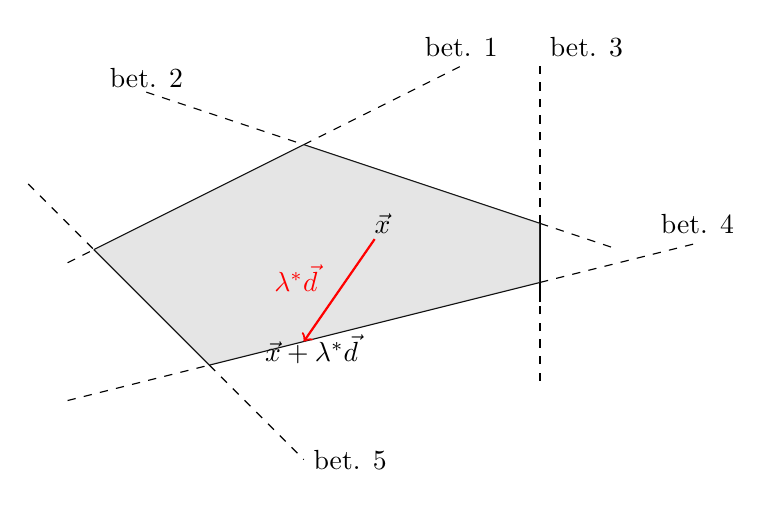
\begin{tikzpicture}[ latex
  s/.style={width=0}]

  %ligning 1
	\draw[domain=-1:-2/3,variable=\x,dashed] 	plot({\x},{0.5*\x+1});
	\draw[domain=-2/3:2,variable=\x] 			plot({\x},{0.5*\x+1});
	\draw[domain=2:4,variable=\x,dashed] 	plot({\x},{0.5*\x+1}) node[above] {bet. 1};
	
  %ligning 2
  	\draw[domain=0:2,variable=\x,dashed] 	plot({\x},{-(1/3)*\x+8/3}) node[above] at (0,2.6) {bet. 2} ;
	\draw[domain=2:5,variable=\x] 			plot({\x},{-(1/3)*\x+8/3});
	\draw[domain=5:6,variable=\x,dashed] 	plot({\x},{-(1/3)*\x+8/3});
	

  %ligning 3
  	\draw[domain=-1:0,variable=\y,dashed] 	plot({5},{\y});
	\draw[domain=0:1,variable=\y] 			plot({5},{\y});
	\draw[domain=1:3,variable=\y,dashed] 	plot({5},{\y}) node[above right] {bet. 3};
	
  %ligning 4
	\draw[domain=-1:4/5,variable=\x,dashed] 	plot({\x},{0.25*\x-1});
	\draw[domain=4/5:5,variable=\x] 			plot({\x},{0.25*\x-1});
	\draw[domain=5:7,variable=\x,dashed] 	plot({\x},{0.25*\x-1}) node[above] {bet. 4};
	
  %ligning 5
  	\draw[domain=-1.5:-2/3,variable=\x,dashed] 	plot({\x},{-\x}) ;
	\draw[domain=-2/3:4/5,variable=\x] 			plot({\x},{-\x});
	\draw[domain=4/5:2,variable=\x,dashed] 	plot({\x},{-\x}) node[right] {bet. 5} ;

  %løsningsmængden skraveret
	\fill[gray!80,nearly transparent] (4/5,-4/5) -- (-2/3,2/3) -- (2,2) -- (5,1) --(5,0.25) --  cycle;
	
  % vektor x
	\node[] (x) at (3,1) {$\vec{x}$};
	\draw[thick, color=red, ->](2.9,0.8) -- (2,-0.5) node[above, yshift=0.5 cm, xshift=-0.1 cm] {$\lambda^* \vec{d}$} ;
	\node[] (x) at (2.1, -0.6) {$\vec{x}+\lambda^* \vec{d}$};
 
\end{tikzpicture}
	\captionof{figure}{Der ligges et multiplum af en retnings vektor til vektor $\vec{x}$ til at summen gør betingelse $4$ aktiv.}
	\label{fig:eksistens}
\end{center}
\end{figure}
Da objektfunktionen til enhver vektor i løsningsmængden, derfor er mindre eller lig objektfunktionen til en mulig basisløsning, må den optimale løsning, være en mulig basisløsning.
\begin{proof}
Da $P$ ikke er tom må der eksistere en vektor $\vec{x} \in P$.
Antag at $\vec{x}$ ikke er en mulig basisløsning, da vil $I = \{i | \vec{a_i}^T\vec{x} = b_i\}$, hvor $\vec{a_i}^T\vec{x}=b_i$ er aktive lineære uafhængige bibetingelser, indeholde færre end $n$ elementer. 
Nu konstrueres en mulig basisløsning $\vec{x^*}$, med udgangspunkt i $\vec{x}$ så $\vec{c}^T\vec{x^*}\leq \vec{c}^T\vec{x}$.
Da $|I|<n $ må $span(\{a_i | i \in I\})$ være et ægte underrum til $\mathds{R}^n$, hvorfor der eksistere en vektor $\vec{d} \in \mathds{R}^n$ så $\vec{a_I}^T\vec{d}=0$ for alle $i \in I$. 
Vælg nu fortegn på $\vec{d}$ så $\vec{c}^T\vec{d} \leq 0$, da vil $\vec{c}^T(\vec{x}+\lambda\vec{d}) \leq \vec{c}^T\vec{x}$ hvor $\lambda$ er en positiv skalar.
Da $P$ er begrænset, og derfor ikke indeholder en linje, må der være et $\lambda'$ som gør, at $\vec{x}+\lambda'\vec{d} \notin P$, hvorfor at der for et $\lambda^*$ må gælde, at $\vec{a_j}^T(\vec{x}+\lambda^* \vec{d}) = b_j$, for $j \notin I$.
Bemærk at $\vec{x}+\lambda^*\vec{d} \in P$, da $\vec{a_i}^T(\vec{x}+\lambda\vec{d})= \vec{a_i}^T\vec{x} = b_i$, for $i \in I$, hvorfor alle aktive bibetingelser stadig er overholdt.
Antag nu at $\vec{d}$ er lineært afhængig af andre bibetingelser end $\vec{a_j}$, da vil $\vec{a_j}$ også være lineært afhæng af dem, hvorfor det følger af Sætning \ref{stn:PQ}, at man kan se bort fra dem, og $\vec{x}+\lambda \vec{d} \in P$ må derfor stadig gøre sig gældende. 
Da $\vec{d}$ er lineært afhængig af $\vec{a_j}$, må det medfører, at da $\vec{d}$ er lineært uafhængig af $\vec{a_i}$ så må $\vec{a_j}$ også være det. 
Derfor kan $j$ tilføjes til $I$. 
Gentag til at $I$ indeholder $n$ lineært uafhængige vektorer, hvorefter det følger af Definition \ref{def:basislosning} at en basisløsning er konstrueret, og da løsningen er konstrueret ud fra en mulig løsning uden at overtræde nogle betingelser, må det være en mulig basisløsning.\\
Da $\vec{x^*}$ er konstrueret ud fra en vilkårlig vektor $\vec{x}\in P$ medføre det, at en mulig basisløsning altid vil opfylde $\vec{c}^T\vec{x^*} \leq \vec{c}\vec{x}$ for en hver ikke mulig basisløsning. 
Da der kun er en endelig mængde mulige basisløsninger, må der være en vektor $\vec{x^{**}}$, som opfylder, at $\vec{c}^T\vec{x^{**}}\leq \vec{c}^T\vec{x^*}$ for alle andre mulige basisløsninger, hvorfor at $\vec{x^{**}}$ er en optimal løsning.
\end{proof}
Sætning \ref{stn:eksistens} kan omskrives en smugle, så i stedet for at kravet er, at løsningsmængden ikke har en linje, så er det at objekt funktionen til løsningsmængden er begrænset.
\begin{kor}
Lad $f(\vec{x}) = \vec{c}^T\vec{x}$ betegne et lineært minimerings programmerings problem, med mulige løsningsmængde $\mathcal{F} \neq \emptyset$. 
Da eksistere en optimal løsning, som er en mulig basisløsning, hvis der eksistere et $K \in \mathds{R}$ så $|f(\mathcal{F})| \leq K$ 
\label{kor:eksistens}
\end{kor}
\begin{proof}
Lad  $K \in \mathds{R}$ så $|f(\mathcal{F})| \leq K$, da må der for et hvert $\vec{x} \in P$ og $\vec{d} \in \mathds{R}^n$ eksistere et $\lambda$ så $f(\vec{x}+\lambda \vec{d}) = K$, og da $f$ er lineær, følger det, at $\mathcal{F}$ ikke kan indeholde en linje. 
Da $\mathcal{F} \neq \emptyset$ følger det af Sætning \ref{stn:eksistens}, at er eksistere en optimal løsning, som er en mulig basisløsning til det lineære minimerings programmerings problem.
\end{proof}
Det betyder, at hvis der til et lineært programmerings problem skal eksistere en optimal løsning, så må løsningsmængden ikke indeholde en linje og objektfunktion på løsningsmængden skal være begrænset. 
Er det ikke tilfældet må objektfunktionen kunne tage værdierne $\infty$ og $-\infty$, og det vil derfor være løsningen på problemet, alt afhængig af om, der er tale om et henholdsvis maksimering eller minimerings problem.




